%%%%%%%%%%%%%%%%%%%%%%%%%%%%%%%%%%%%%%%%%%%%%%%%%%%%%%%%%%%%%%%%%%%%%%%%%%%%%%%%
% Inicializálás                                                                %
%%%%%%%%%%%%%%%%%%%%%%%%%%%%%%%%%%%%%%%%%%%%%%%%%%%%%%%%%%%%%%%%%%%%%%%%%%%%%%%%

%%%%%%%%%%%%%%%%%%%%%%%%%%%%%%%%%%%%%%%%%%%%%%%%%%%%%%%%%%%%%%%%%%%%%%%%%%%%%%%%
% Papírméret, betűméret, margó, magyar karakterek                              %
%%%%%%%%%%%%%%%%%%%%%%%%%%%%%%%%%%%%%%%%%%%%%%%%%%%%%%%%%%%%%%%%%%%%%%%%%%%%%%%%

\documentclass[a4paper,12pt]{article}
\special{papersize=210mm,297mm}

\usepackage{anysize}
\marginsize{2.5cm}{2.5cm}{2.5cm}{2.5cm}

\usepackage[utf8]{inputenc}
\usepackage[magyar]{babel}

%%%%%%%%%%%%%%%%%%%%%%%%%%%%%%%%%%%%%%%%%%%%%%%%%%%%%%%%%%%%%%%%%%%%%%%%%%%%%%%%
% Fedlap inicializálása                                                        %
%%%%%%%%%%%%%%%%%%%%%%%%%%%%%%%%%%%%%%%%%%%%%%%%%%%%%%%%%%%%%%%%%%%%%%%%%%%%%%%%

\usepackage{fedlap}

\csapat{unexpected\_exceptions}{59}
\konzulens{Ferencz Endre}

\taga{Biró Loránd}{NCZAGL}{lol.kylerrr@gmail.com}
\tagb{Kanyó Tibor}{NXWUKE}{kanyo.tibi@gmail.com}
\tagc{Magyar Dániel}{SUFFGT}{samuraidanm@gmail.com}
\tagd{Tarjáni Tamás}{S499KV}{tarjanitomi@gmail.com}
\tage{Vajsz Kornél}{VUYNAW}{roncsipar@gmail.com}

%%%%%%%%%%%%%%%%%%%%%%%%%%%%%%%%%%%%%%%%%%%%%%%%%%%%%%%%%%%%%%%%%%%%%%%%%%%%%%%%
% Fejléc és lábléc                                                             %
%%%%%%%%%%%%%%%%%%%%%%%%%%%%%%%%%%%%%%%%%%%%%%%%%%%%%%%%%%%%%%%%%%%%%%%%%%%%%%%%

\usepackage{fancyhdr}

\setlength{\headheight}{1.4em}
\setlength{\headsep}{2em}

\fancyhf{}
\fancyhead[OL] { \leftmark{} }
\fancyhead[OR] { \tmpcsapat }
\fancyfoot[OC] { \thepage }
\fancyfoot[OR] { \tmpdatum }

\pagestyle{fancy}

%%%%%%%%%%%%%%%%%%%%%%%%%%%%%%%%%%%%%%%%%%%%%%%%%%%%%%%%%%%%%%%%%%%%%%%%%%%%%%%%
% Napló                                                                        %
%%%%%%%%%%%%%%%%%%%%%%%%%%%%%%%%%%%%%%%%%%%%%%%%%%%%%%%%%%%%%%%%%%%%%%%%%%%%%%%%

\usepackage{longtable}

\newenvironment{journal}
{
	\hbadness 10000
	\begin{longtable}{|p{60pt}|l|l|p{216pt}|}
	\hline
	\textbf{Kezdet} & \textbf{Időtartam} & \textbf{Résztvevők} & \textbf{Leírás} \\
	\hline
	\endfirsthead
	\hline
	\textbf{Kezdet} & \textbf{Időtartam} & \textbf{Résztvevők} & \textbf{Leírás} \\
	\hline
	\endhead
}
{
	\end{longtable}
}

\newcommand{\journalentry}[4]
{
	{#1} & {#2} óra & \parbox{50pt}{#3} & {#4} \\
	\hline
}

%%%%%%%%%%%%%%%%%%%%%%%%%%%%%%%%%%%%%%%%%%%%%%%%%%%%%%%%%%%%%%%%%%%%%%%%%%%%%%%%
% UseCase leírás                                                               %
%%%%%%%%%%%%%%%%%%%%%%%%%%%%%%%%%%%%%%%%%%%%%%%%%%%%%%%%%%%%%%%%%%%%%%%%%%%%%%%%

\newenvironment{usecase}
{
	\hbadness 10000
	\begin{longtable}[l]{|p{100pt}|p{328pt}|}
	\hline
	\endfirsthead
	\hline
	\endhead
}
{
	\hline
	\end{longtable}
}

\newcommand{\usecaseentry}[2]
{
	\hline
	\textbf{#1} & {#2}\\
}

%%%%%%%%%%%%%%%%%%%%%%%%%%%%%%%%%%%%%%%%%%%%%%%%%%%%%%%%%%%%%%%%%%%%%%%%%%%%%%%%
% FileList leírás                                                               %
%%%%%%%%%%%%%%%%%%%%%%%%%%%%%%%%%%%%%%%%%%%%%%%%%%%%%%%%%%%%%%%%%%%%%%%%%%%%%%%%

\newenvironment{filelist}
{
	\hbadness 10000

	\begin{longtable}{|p{145pt}|p{35pt}|p{63pt}|p{163pt}|}
	\hline
	\textbf{Fájl neve} & \textbf{Méret} & \textbf{Keletkezés ideje} & \textbf{Tartalom} \\
	\hline
	\endfirsthead
	\hline
	\textbf{Fájl neve} & \textbf{Méret} & \textbf{Keletkezés ideje} & \textbf{Tartalom} \\
	\hline
	\endhead
}
{
	\end{longtable}
}

\newcommand{\filelistentry}[4]
{
	{#1} & {#2} b & {#3} & {#4} \\
	\hline
}
%%%%%%%%%%%%%%%%%%%%%%%%%%%%%%%%%%%%%%%%%%%%%%%%%%%%%%%%%%%%%%%%%%%%%%%%%%%%%%%%
% Egyebek                                                                      %
%%%%%%%%%%%%%%%%%%%%%%%%%%%%%%%%%%%%%%%%%%%%%%%%%%%%%%%%%%%%%%%%%%%%%%%%%%%%%%%%

\usepackage{graphicx}		% Kepek beillesztesehez
\usepackage{epstopdf}		% EPS fajlok felismeresehez
\graphicspath{{Images/}}	% Az Images mappaban keresse a kepeket

\anyag{2. Követelmény, projekt, funkcionalitás}
\datum{2012. február 19.}
\setcounter{section}{1}

%%%%%%%%%%%%%%%%%%%%%%%%%%%%%%%%%%%%%%%%%%%%%%%%%%%%%%%%%%%%%%%%%%%%%%%%%%%%%%%%
% Dokumentum                                                                   %
%%%%%%%%%%%%%%%%%%%%%%%%%%%%%%%%%%%%%%%%%%%%%%%%%%%%%%%%%%%%%%%%%%%%%%%%%%%%%%%%

\begin{document}

\fedlap

\section{Követelmény, projekt, funkcionalitás}

\subsection{Követelmény definíció}

\subsubsection{A program célja, alapvető feladatai}

A program egy játék, melyben egy avatárt kell irányítani, akinek feladata, hogy megszerezze a kulcsot, majd a bezárt ajtóhoz eljusson. A játékot kétféle kameranézetből követhetjük figyelemmel: közeli és távoli. A távoli módban, kirakószerűen a több elemből álló pályarészleteket kell mozgatnunk, hogy ezáltal kialakíthassuk az útvonalunkat célunk eléréséhez. A közeli módban az avatárra ráközelítve, őt magát irányíthatjuk néhány pályaelemen keresztül. Bővebb részleteket a Feladatleírás című rész tartalmaz.

\subsubsection{A felhasználói felület}

A kész játék grafikus felhasználói felülettel fog rendelkezni, amely billentyűzet és egér felhasználásával lesz irányítható. A felületet a távoli kameranézetben a pályaelemek sokasága, közeli kameranézetben pedig egynéhány pályaelem és az avatár fogják elfoglalni játék közben.

\subsubsection{A program futtatásához szükséges követelmények}

A futtatáshoz szükséges, hogy a felhasználó számítógépére telepítve legyen a Java Runtime Environment (JRE) 1.6-os verziója, mivel böngészőből futtathatónak készül. A most használt PC-k nagy részén zökkenőmentesen fut, hiszen a futtatáshoz szükséges követelmények megegyeznek az előírt JRE verzió mindenkori követelményeivel, ennek ellenére az optimális futtatáshoz legalább P4 1GHz-es processzorral, 512 MB rammal és 200 MB lemezterülettel, billentyűzettel, egérrel rendelkező géppel kell rendelkezni.

\subsubsection{A fejlesztőkörnyezet}

A fejlesztéshez Eclipse-t használunk, s UMLet programmal modellezünk, majdan ez alapján generáljuk a kód vázát. Verziókövetéshez SVN-t alkalmazunk.  Teszteléshez a JUnitot fogjuk használni. A dokumentumokat LaTex nyelven készítjük a MikTex-et használván.

\subsubsection{Minőségi tényezők}

Ezen tulajdonságok közül kiemelném a legfontosabbakat, amiket egy mai szoftvertől elvárunk, hogy teljesítsen.

\textbf{Teljesítmény}: A cél az, hogy a játék megfelelő kikapcsolódást nyújtson a felhasználó-nak. Ebből kifolyólag folyamatosan szem előtt tartjuk a fejlesztés során, hogy oly hangulati világot, élményt teremtsünk, amit élvezni tud majd.

\textbf{Újrafelhasználhatóság}: Ennek célja, hogy olyan programot hozzunk létre az Objektum Orientált szemléletnek megfelelően, melyet később könnyedén lehessen módosítani, illetve kisebb változtatások után integrálni lehessen más alkalmazásokba.

\textbf{Rugalmasság}: Ez a fejlesztőkörnyezetből, illetve abból, hogy alapkövetelmény, hogy a program minden olyan környezetben elfusson, ahol létezik Java futtatókörnyezet egyszerűnek mondható.

\textbf{Felhasználhatóság}: Szem előtt tartjuk mindenkor azt a célt, hogy a játékot olyan emberek is képesek legyenek élvezni, akik a számítástechnikában nem rendelkeznek magasfokú tapasztalattal. Természetesen azt a szintet elvárjuk, ami a játék elindításához szükségeltetik.

\subsubsection{A szoftver minősítése}

A végső verziója a szoftvernek akkor megfelelő, ha teljesíti a fentebb leírtakat. Ezek ellenőrizhetők a játék futtatásával, valamint a kód és a modell összehasonlításával.

\subsubsection{A kibocsátás}

A játék kibocsátása a konzulens előtt fog megtörténni mellékelve a dokumentációt és a forráskódot. Az ellenőrzést és az értékelést követően elérhetővé válik majdan az interneten is.

\subsection{Projekt terv}

\subsubsection{A fejlesztői csapat}
\begin{tabular}{|l|l|}
\hline 
\textbf{Név} & \textbf{Elsődleges feladatkör} \\ 
\hline 
Bíró Lóránd & Kód \\ 
\hline 
Kanyó Tibor & Dokumentáció \\ 
\hline 
Magyar Dániel & Csapatvezető, Dokumentáció, Nyomtatás \\ 
\hline 
Tarjáni Tamás & Dokumentáció \\ 
\hline 
Vajsz Kornél & Kód \\ 
\hline 
\end{tabular} 

\subsubsection{Életciklus modell}
	A projekt jelen, specifikációs fázisát követő lépés az \textbf{analízis modell }, mely magában foglalja a struktúra- és viselkedési diagramok megfelelő kidolgozását. Ez a fázis kiemelke-dően fontos szerepet játszik a projekt életciklusában. 

	A helyes modell kidolgozását, és ellenőrzését követő lépés a \textbf{szkeleton tervezése és beadása}, ami a korrekt modellek és a szükséges programozási tudás ismeretében, nem jelenthet különösebb problémát a csapatnak.
	
	A következő lépés a \textbf{prototípus tervezése és implementálása}kor, a programnak könnyen tesztelhetőnek kell lennie, hogy a programozási és esetleges logikai hibák könnyen felismerhetőek legyenek.
	
	A projekt következő, és egyben utolsó fázisa a \textbf{grafikus felület megvalósítása}, amit követően a végleges dokumentációt és forráskódokat leadjuk.
	
\subsubsection{Szervezési struktúra}
	Az öt fős csapat tagjai többnyire eltérő ismeretekkel rendelkezik a szoftverfejlesztés területén, az aktuális részfeladatok kiosztásánál így kiemelt hangsúlyt fektetünk az egyéni preferenciákra, érdeklődésre. A feladat felosztását, megoldandó problémák átbeszélését a hivatalos konzultáció fennmaradó idejében,\textbf{ minden szerdán 12.00-14.00} időpontban, ennek rövidsége esetén \textbf{szerda 18.00 után}, mind az öt fő jelenlétében végezzük. Ezen találkozók alkalmával a csapat tagjai az egyes részfeladatok egymásra épülése miatt, esetleg különböző határidők betartásában egyezik meg.
	A csapat, a személyes konzultációkon kívül a folyamatos kapcsolattartás érdekében elsődlegesen privát levelező listát használ, sürgősebb esetekben pedig skype-on, illetve telefonon vesszük fel egymással a kapcsolatot.
	
\subsubsection{Fejlesztési ütemterv}
A szoftver fejlesztésének három fő lépcsőfoka
	\textbf{1. Szkeleton:} Célja az objektum és dinamikus modellek ellenőrzése. Csak az interfészek kerülnek definiálásra, illetve a metódu-sok szöveges formában kiírják a saját nevüket, majd meghívja a szükséges metódusokat. Amennyiben szükséges, az interaktivitás a képernyőn karakteres formában feltett kérdés és a felhasználó (tesztelő) által adott válasz függvényében történik.
	\textbf{2. Prototípus:} A program célja a funkcionalitás betöltésének bizonyítása, grafikus interfész nélkül, azaz minden  a megjelenítéstől független business objektum a végleges algoritmusokat tartalmazza. A megjelenítés és működtetés alfanumerikus képernyőn történik, illetve fájlba menthető, így megteremtve a rendszer szintű tesztelés lehetőségét. Különös figyelemmel kell eljárni az interfész felépítésekor.
	\textbf{3. Grafikus változat:} A prototípustól csupán a kezelői felület minőségében eltérő program.

\subsubsection{Határidők}
\begin{tabular}{|c|l|}
\hline 
\textbf{Dátum} & \textbf{Feladat} \\ 
\hline 
febr. 10. & Csapat regisztráció \\ 
\hline 
febr. 20. & Követelmény, projekt, funcionalitás -  beadás \\ 
\hline 
febr. 27. & Analízis modell kidolgozása 1. -  beadás \\ 
\hline 
márc. 5. & Analízis modell kidolgozása 2. -  beadás \\ 
\hline 
márc. 12. & Szkeleton tervezése - beadás \\ 
\hline 
márc. 19. & Szkeleton - beadás \\ 
\hline 
márc. 26. & Prototípus koncepciója - beadás \\ 
\hline 
ápr. 2. & Részletes tervek - beadás \\ 
\hline 
ápr. 16. & Prototípus - beadás \\ 
\hline 
ápr. 23. & Grafikus felület specifikációja - beadás \\ 
\hline 
máj. 7. & Grafikus változat - beadás \\ 
\hline 
máj. 11. & Összefoglalás - beadás \\ 
\hline 
\end{tabular} 

\subsubsection{Kockázatok}

\begin{tabular}{|c|c|c|}
\hline 
\textbf{Esemény} & \textbf{Valószínűség} & \textbf{Hatás} \\ 
\hline 
csapattag kilépése & mérsékelt & súlyos \\ 
\hline 
hardware hiba & kicsi & elviselhető \\ 
\hline 
követelmény változás & nagyon magas & nem jelentős \\ 
\hline 
határidőből való kicsúszás & kicsi & súlyos \\ 
\hline 
csapattag lebetegedése & mérsékelt & elviselhető \\ 
\hline 
kommunikációs  problémák & kicsi & súlyos \\ 
\hline 
\end{tabular} 
\subsection{Feladatleírás}

A feladatunk elkészíteni egy több pályából álló fejtörő (ún. puzzle) játékot, amelyben a játékos célja az egyes pályákon az általa irányított avatárral megszerezni a kijárathoz tartozó kulcsot, majd eljutni a kijárathoz.\medskip

A programot elindítva a játékost egy menü üdvözli, itt néhány egyszerű menüpont közül választhat: Új játék, Játék folytatása illetve Súgó. Az Új játék menüpont értelem-szerűen teljesen új játékot indít, az esetleg korábban megkezdett játék elveszik. A Játék folytatása gombra kattintva lehetőségünk van a korábban megkezdett játékunkat a legutolsó mentett helyen folytatni, míg a Súgó menüpont alatt a játék irányítását ismerhetjük meg, és a játékmenettel kapcsolatban találunk segítséget.\medskip

Ha elindítunk egy új, vagy már megkezdett játékot, akkor az adott (az első vagy az éppen következő) pálya távoli kameranézetébe érkezünk. Ez lényegében a jól ismert "tili-toli" játék, aminek lényege: van valamennyi üres helyünk, ezeket egy hely kivételével valamilyen (számokat, egy kép darabjait, esetünkben pályaelemeket ábrázoló) lapokkal lefedjük. A játékos az éppen aktuális üres hellyel szomszédos lapok közül valamelyiket az üres helyre mozgatja, ennek a lapnak az előző tartózkodási helye felszabadul, üres hellyé válik, ahova ismét mozgathatunk lapot az ő szomszédjai közül. Ezt a lépést ismételve törekszünk valamilyen cél (a számok sorba rendezése, a kép kirakása vagy a pálya kedvezőbb elrendezése) elérésére. A programban az egyes lapok a pálya egyes elemeit tartalmazzák, ezeket az előbb megismert módon szabadon mozgathatjuk. Ezek közül a pályaelemek közül valamelyik tartalmazza a kijárat kinyitásához szükséges kulcsot, egy (jellemzően másik pályaelemen) a kijáratot jelképező ajtót, és valamelyikben megtalálható az avatárunk, akit ki szeretnénk juttatni a pályáról. A távoli kameranézetben nincs lehetőségünk őt irányítani, ehhez egy másik kameranézetbe kell váltanunk.\medskip

A távoli kameranézetből egy gomb lenyomásával átkerülünk a közeli kameranézetbe, ekkor csak egy vagy kettő pályaelem látszik: az, amelyik az avatárt tartalmazza, és esetleg egy szomszédos pályaelem is. A középpontba az avatár kerül, most már lehetőségünk nyílik irányítani őt. Képes jobbra és balra futni, ugrani, illetve ezek kombinációjaként valamelyik irányba ferdén felfelé ugrani. Egy pályaelemen belül ezeket minden gond nélkül megteheti, pályaelemek között azonban csak akkor tud közlekedni, ha azok tökéletesen összeillenek (ugyanolyan magasan kezdődik a föld az egyiken, mint amilyen magasan a másikon befejeződött). Ha ez nem teljesül, tehát egy nem illeszkedő pályaelembe szeretnénk átjutni, akkor falba ütközünk, nem tudunk továbbmenni. Ezt nincs lehetőség ugrással sem kijátszani, hiába tudnánk felugrani olyan magasra, ahol a másik pályaelem kezdődik, a játék ezt nem engedi meg – kénytelenek leszünk illeszkedő pályaelemeket egymás mellé mozgatni. Amennyiben vissza szeretnénk váltani a távoli kameranézetbe, a nézetváltó gomb ismételt megnyomásával ezt könnyedén megtehetjük, így ismét kedvünkre rendezhetjük a pályaelemeket, új utakat nyitva meg az avatárunk előtt.\medskip 

A pálya befejezéséhez először a kulcsot kell megszereznünk, majd el kell jutnunk a kijárathoz. A kijutáshoz mindenképpen szükségünk van a kulcsra, anélkül ugyanis nem tudjuk kinyitni az ajtót. Ha befejeztünk egy pályát, akkor a program tájékoztat minket, hogy hol járunk: megtudhatjuk az éppen befejezett pálya sorszámát, és hogy mennyi pálya van még hátra a játékból. Ezután tetszőleges gomb lenyomásával a következő pálya távoli kameranézetébe érkezünk, a feladatunk ugyanúgy a kulcs megszerzése és az ajtó elérése. A játék akkor ér véget, ha a játékos az utolsó pályáról is sikeresen kijutott.\medskip

A játékot nem szükséges egy nekifutásra befejezni, akármikor lehetőségünk van ki-lépni. A program megjegyzi, hogy hol tartunk éppen, és legközelebb a menüben Játék folytatása lehetőséget választva a következő, még be nem fejezett pályán tehetjük próbára képességeinket.

\subsection{Szótár}

\begin{description}

\item[játékos]
A számítógépet és a játékszoftvert használó és irányító személy.

\item[játékablak]
Az a terület a képernyőn, ahol a játékszoftver megjeleníti a játékot.

\item[avatár]
A virtuális megtestesítése a \emph{játékosnak} akit irányíthatunk, esetünkben ez egy pálcikaember.

\item[input]
\emph{Input-nak} nevezzük a \emph{játékos} "utasításait", amit a játékszoftver értelmezni tud. Ide tartoznak a billentyűleütések, az egérkattintások, vagy akár csak az egér mozgatása.



\item[pályaelem]
Különböző módon elrendezett falakból, padlókból és alakzatokból álló egység méretű tér ahol az \emph{avatár} mozoghat. A \emph{játékos} ennek a térnek csak egy négyzet alakú síkmetszetét látja, csak ebben a síkmetszetben mozoghat az \emph{avatárral}.

\item[illeszkedő pályaelemek]
Két különböző \emph{pályaelem} akkor és csak akkor illeszkedik, ha közvetlenül egymás mellett (vagy felett/alatt) vannak, tehát osztoznak egy élen, és a két pályaelem közös élét érintő falainak, padlóinak és alakzatainak határvonalai a közös élt metsző szakaszokra egészítik ki egymást.

\item[kulcs]
Az a kulcsként megjelenített téglalap alakú hely egy \emph{pályaelemen} belül, ahova az \emph{avatárt} eljuttatva az \emph{avatár} "felveszi" a kulcsot. Ha az \emph{avatár} felvette, avagy birtokában van a \emph{kulcsnak} további lehetőségei nyílnak meg. Ekkor a \emph{kulcs} eltűnik a \emph{pályaelemről}.

\item[kijárat]
Az az ajtóként megjelenített téglalap alakú hely egy \emph{pályaelemen} belül, ahova az \emph{avatárt} eljuttatva az aktuális feladvány megoldottnak számít. Ennek feltétele, hogy az \emph{avatárnál} van a \emph{kulcs}. Ezt a helyet egy ajtó szimbolizálja.

\item[pálya]
Egy \emph{pálya} egy feladványnak felel meg, ami bizonyos számú előre meghatározott rácsos elrendezésű \emph{pályaelemekből} áll. Minden pályán pontosan egy \emph{kulcs} és egy \emph{kijárat} található.

\item[játék]
A \emph{pályák}, vagyis a feladványok sorrendben való megoldásának folyamatát hívjuk \emph{játéknak}.



\item[kameranézet]
A különböző \emph{kameranézetek} vezérlik, hogy a \emph{pálya} a \emph{játékablakban} való elhelyezéséből adódóan mely részei láthatóak, és ez a látható terület hogyan változik a \emph{játékos} \emph{input}jaira, továbbá azt, hogy a játékszoftver milyen \emph{input}okra reagál és hogyan.

\item[távoli kameranézet]
Ebben a \emph{kameranézetben} a teljes \emph{pálya} látható és a \emph{játékosnak} csak a \emph{pályaelemek} mozgatására van lehetősége.

\item[közeli kameranézet]
Ebben a \emph{kameranézetben} a \emph{pálya} úgy van megjelenítve, hogy végig az \emph{avatár} van a \emph{játékablak} középpontjában és éppen csak valamely szomszédos \emph{pályaelemre} van rálátásunk. Ekkor csak az \emph{avatárunk} irányítására van lehetősége a \emph{játékosnak}.



\item[menü]
A játékos pillanatnyi lehetőségeit összefoglaló felület, ahonnan többek között a \emph{játékot} tudjuk elindítani.

\end{description}

\subsection{Essential use-case-ek}

\subsubsection{Use-case diagram}
\begin{figure}[htb]
\centering
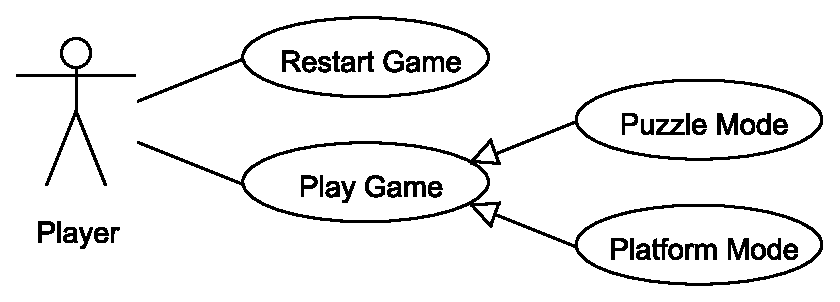
\includegraphics[scale=0.7]{02_General.eps}
\caption{Az első use-case diagram}
\label{fig:02general}
\end{figure}

\subsubsection{Use-case leírások}
\begin{center}
\begin{tabular}{|l|p{320pt}|}
\hline 
\textbf{Use-case neve} & Restart Game \\ 
\hline \hline
\textbf{Rövid leírás} & Új játék indítása. \\ 
\hline 
\textbf{Aktorok} & Player \\ 
\hline 
\textbf{Forgatókönyv} & A játék újraindul. Az eddigi eredmények elvesznek. \\ 
\hline
\end{tabular}
\end{center}

\begin{center}
\begin{tabular}{|l|p{320pt}|}
\hline 
\textbf{Use-case neve} & Play Game \\ 
\hline \hline
\textbf{Rövid leírás} & A megkezdett játék folytatása. Egyébként új játék indítása. \\ 
\hline 
\textbf{Aktorok} & Player \\ 
\hline 
\textbf{Forgatókönyv} & Elindul a játék Puzzle Mode-ban. A képernyőn kirajzolódik az utolsó megkezdett pálya. \\ 
\hline
\end{tabular}
\end{center}

\begin{center}
\begin{tabular}{|l|p{320pt}|}
\hline 
\textbf{Use-case neve} & Platform Mode \\ 
\hline \hline
\textbf{Rövid leírás} & A játékos utasításokkal irányíthatja a pálcikaembert. \\ 
\hline 
\textbf{Aktorok} & Player \\ 
\hline 
\textbf{Forgatókönyv} & A játékos nyilakkal irányíthatja a pálcikaembert. Space billentyűre a Platform Mode szünetel, a program átlép Puzzle Mode-ba. \\ 
\hline
\end{tabular}
\end{center}

\begin{center}
\begin{tabular}{|l|p{320pt}|}
\hline 
\textbf{Use-case neve} & Puzzle Mode \\ 
\hline \hline
\textbf{Rövid leírás} & A játékos utasításokkal mozgathatja a kirakót. \\ 
\hline 
\textbf{Aktorok} & Player \\ 
\hline 
\textbf{Forgatókönyv} & A játékos nyilakkal tologathatja a kirakó elemeit. Space billentyűre a Puzzle Mode szünetel, a program átlép Platform Mode-nak abba az elembe ahol a pálcikaember található. \\ 
\hline
\end{tabular}
\end{center}

%%%%%%%%%%%%%%%%%%%%%%%%%%%%%%%%%%%%%%%%%%%%%%%%%%%%%%%%%%%%%%%%%%%%%%%%%%%%%%%%
% Napló                                                                        %
%%%%%%%%%%%%%%%%%%%%%%%%%%%%%%%%%%%%%%%%%%%%%%%%%%%%%%%%%%%%%%%%%%%%%%%%%%%%%%%%

\newpage
\subsection{Napló}

\begin{journal}

\journalentry{2012.02.15. 12:00}{1,5}{Biró Kanyó Magyar Tarjáni Vajsz}{Értekezlet: megbeszéltük, hogy SVN szerveren keresztül fog menni a munka.}

\journalentry{2012.05.15. 15:00}{1}{Vajsz}{Elkészítettem az Essential Use-Case-eket és beraktam egy dokumentumsablonba.}

\journalentry{2012.02.15. 18:00}{1,5}{Biró}{Megvizsgáltam a Windows-on elérhető \LaTeX{} szerkesztőket és beüzemeltem, bekonfiguráltam a csapat SVN szerverét, írásban beszámoltam minderről a csapatnak.}

\journalentry{2012.02.15. 18:11}{1,5}{Kanyó}{A programmal szemben felállított követelményeket fogalmaztam meg. Majdnem mindegyik pontot kifejtettem teljesen.}

\journalentry{2012.02.16. 23:00}{2}{Biró}{Rendszereztem és letisztáztam az eddig elkészült \LaTeX{} kódot, újraszerveztem az SVN könyvtárszerkezetet, megvalósítottam a fedlapot \LaTeX{}-ben, írásban beszámoltam.}

\journalentry{2012.02.17. 11:00}{1,5}{Vajsz}{Összehasonlítottam a Visual Studio, a Soyatec eUML, valamint a Papyrus UML modellező szolgáltatásait, majd tapasztalataimat megosztottam a csapatunk levelezőlistáján.}

\journalentry{2012.02.17. 12:40}{0,5}{Kanyó}{A követelmények fejezetben a már meglévő részeket megformáztam, és javítottam a megfogalmazáson.}

\journalentry{2012.02.17. 14:00}{3}{Tarjáni}{Megírtam a Feladatleírás című fejezetet. Ezt követően ellenőriztem, kisebb javításokat végeztem rajta és beleformáztam a \LaTeX{} dokumentumba.}

\journalentry{2012.02.17. 17:00}{2,5}{Biró}{Megvalósítottam a fejlécet és láblécet \LaTeX{}-ben és különböző UML editorokat töltöttem le és vizsgáltam meg (VioletUML, Papyrus, AgroUML, Soyatec eUML2, UMLet). Végül írásban megosztottam tapasztalataimat a csapattagokkal.}

\journalentry{2012.02.17. 18:00}{1,5}{Magyar}{Csapattagok, és feladatok táblázat kitöltése, dokumentum elolvasása, első tétova lépések megtétele \LaTeX{}-ben.}

\journalentry{2012.02.17. 19:50}{1}{Kanyó}{A követelmények részhez megírtam a Minőségi tényezők, Minősítés és Kibocsátás szekciót. Létrehoztam a napló táblázatát.}

\journalentry{2012.02.17. 24:00}{2,5}{Magyar}{A projektterv szekció megírása.}

\journalentry{2012.02.18. 11:00}{4}{Biró}{Megszüntettem \LaTeX{}-ben a warning-okat, megformáztam a naplót, formáztam a kódot néhány helyen, egységesítettem a kifejezéseket és elkészítettem a szótárat.}

\journalentry{2012.02.18. 22:15}{1,5}{Vajsz}{A dokumentumsablonból átvittem az Use-Case leírásokat a \LaTeX{} munkafájlba.}

\journalentry{2012.02.18. 17:50}{0,5}{Tarjáni}{A dokumentum teljes szövegét átolvastam, helyesírási és stilisztikai hibákat javítottam.}

\end{journal}

\end{document}
